\documentclass[t, 14pt, aspectratio=1610]{beamer}
 % align text inside frame to t=top, b=bottom, c=center
 % 8pt, 9pt, 10pt, 11pt, 12pt, 14pt, 17pt, 20pt available as text font
 % select your aspect ratio 4:3=43, 16:9=169, 16:10=1610

\usetheme{Juelich}

%\usetheme{default}
%\usecolortheme{beaver}

\setbeamertemplate{caption}[numbered]
\setbeamertemplate{caption label separator}{:}
\setbeamertemplate{slide counter}[showall]
\setbeamercolor{code}{fg=black,bg=fzjblue!10}
\setbeamercolor{prototype}{fg=black,bg=fzjgreen!20}

\setbeamertemplate{footline}{%
\hfill\usebeamertemplate***{navigation symbols}
\hspace{-1cm}\small\insertframenumber{}/\inserttotalframenumber}


% \setbeamertemplate{footer element1}[default][\insertsection]%

\usepackage{graphics}
\newcommand{\gfxpath}{../images}

\usepackage[ngerman,english]{babel}
%\selectlanguage{ngerman}
\selectlanguage{english}
\usepackage[utf8]{inputenc}
\usepackage[T1]{fontenc}
% =====================================================
%  packages / definitions needed by pandoc
%
\usepackage{xcolor}
\usepackage{fancyvrb}
\usepackage{framed}
\usepackage{longtable}
\usepackage{booktabs}
\usepackage[warn]{textcomp}
% package listings important for code highlighting !
\usepackage{listings}

\providecommand{\tightlist}{%
  \setlength{\itemsep}{0pt}\setlength{\parskip}{0pt}}

%\renewcommand{\emph}[1]{\structure{#1}}

\renewcommand{\thefootnote}{}

% AUTHOR AND TITLE FOR TITLE PAGE
\author[M. Cherti]{Mehdi Cherti}
\institute[JSC]{Cross Sectional Team Deep Learning, Helmholtz AI @ JSC}
\date{2021-05-07}
\title{Day 5: Generative models, Generative Adversarial Networks (GANs) basics}
% \subtitletest{}

%\AtBeginPart{%
%  \subtitle{\partname}
%  \makepart
%  \begin{frame}
%  \frametitle{Outline}
%  \tableofcontents[hideallsubsection]
%  \end{frame}
%}

%\AtBeginSection{%
%  \subtitle{\sectionname}
%  \begin{frame}
%  \frametitle{Outline}
%  \tableofcontents[currentsection]
%  \end{frame}
%}

% -- INCLUDE BACKGROUND GRAPHIC FOR TITLE PAGE
% \titlegraphic{\includegraphics[width=\paperwidth]{../Abbildungen/juwels_cluster_booster_banner}}


\begin{document}
% Titelseite
\fzjset{title page=image}

%\fzjset{title page=text}
\maketitle

%\begin{frame}
%  \frametitle{Outline}
%  \tableofcontents
%\end{frame}

%% pandoc generated slides
\begin{frame}{Generative Models}
\protect\hypertarget{generative-models}{}

\begin{itemize}
\tightlist
\item
  Impressive progress in last years, algorithmic/architectural
  improvements coupled with large scale training
\item
  Lot of different applications: image generation, text generation,
  speech synthesis, and more
\end{itemize}

\center{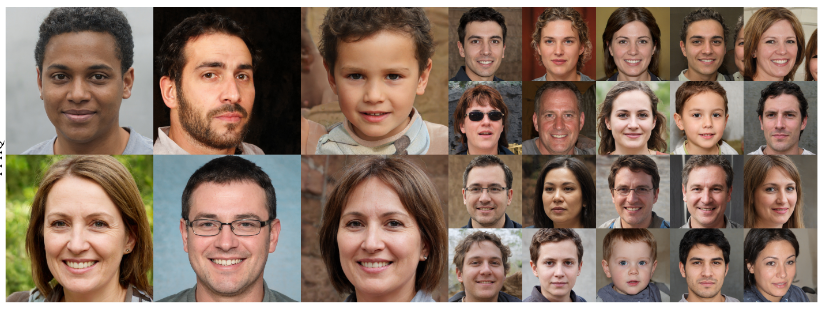
\includegraphics[width=0.8\textwidth]{images/generated_ffhq_karras2020.png}}

Karras et al. (2020)

\end{frame}

\begin{frame}{Generative Models}
\protect\hypertarget{generative-models-1}{}

\begin{itemize}
\tightlist
\item
  Impressive progress in last years, algorithmic improvements coupled
  with large scale training
\item
  Lot of different applications: image generation, text generation,
  speech synthesis, and more
\end{itemize}

\center{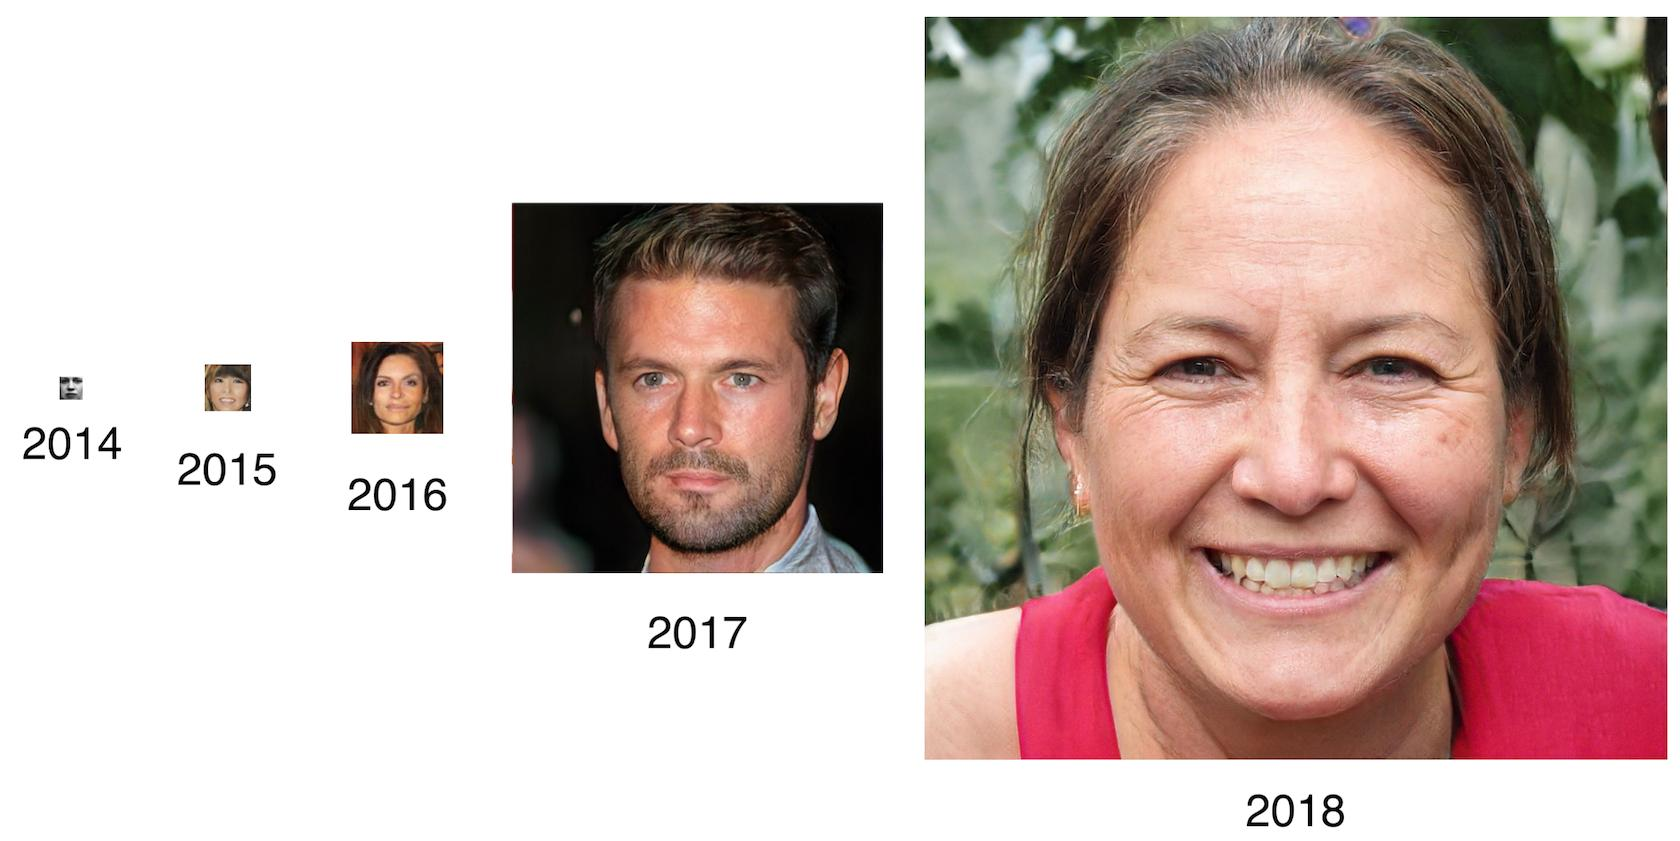
\includegraphics[width=0.68\textwidth]{images/gan_evolution.jpeg}}

(Source: \url{https://bit.ly/3azTV7J})

\end{frame}

\begin{frame}{Generative Models: basics}
\protect\hypertarget{generative-models-basics}{}

\begin{itemize}
\tightlist
\item
  The general setup: we have a set of samples \(x_1,x_2,...,x_N\) drawn
  i.i.d. from an unknown probability distribution \(p(x)\). We would
  like to learn a model \(M\), which we can use to generate samples from
  \(p\)
\item
  Different formulations, training algorithms, architectures
\end{itemize}

\center{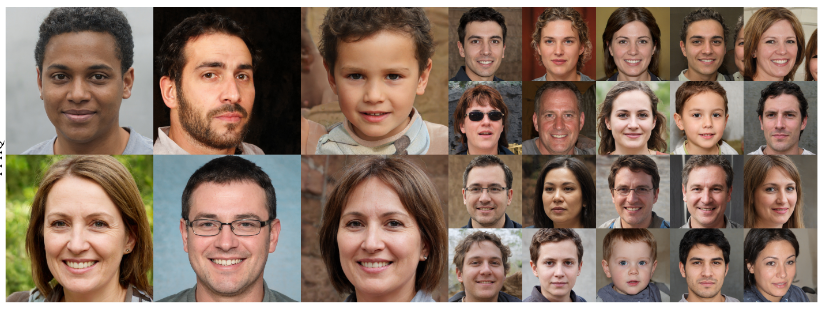
\includegraphics[width=0.8\textwidth]{images/generated_ffhq_karras2020.png}}

Karras et al. (2020)

\end{frame}

\begin{frame}{Generative Models, Density Modeling}
\protect\hypertarget{generative-models-density-modeling}{}

\begin{itemize}
\tightlist
\item
  We model the underlying data distribution of the data \(p(x)\) with a
  surrogate distribution \(q(x)\), i.e. \(q(x) \thickapprox p(x)\) for
  some similarity between probability distributions
\item
  In generative modeling, \(x\) is in general a high-dimensional vector
  (e.g.~image, sound, text)
\item
  A common similarity measure used is the Kullback--Leibler
  (\(\text{KL}\)) divergence:
  \[ D_{\text{KL}} (p \parallel q) = \int p(x)\log\frac{p(x)}{q(x)}dx \]
\end{itemize}

\end{frame}

\begin{frame}{Generative Models, KL Divergence}
\protect\hypertarget{generative-models-kl-divergence}{}

\begin{itemize}
\tightlist
\item
  Connection to information theory and compression:\\
  \(D_{\text{KL}} (p \parallel q) = (-\int p(x)\log q(x)dx) - (-\int p(x)\log p(x)dx) = H(p, q) - H(p)\)
\item
  Connection to maximum likelihood: For a parametrized model
  \(q_{\Theta}\), maximization of the likelihood
  \[ \text{max}_{\Theta}[E_{x \sim p} \log q_{\Theta}(x)] \thickapprox \sum_i \log q_{\Theta}(x_i),\ x_i \sim p \]
  is equivalent to minimizing the \(\text{KL}\) divergence between
  \(q_{\Theta}\) and \(p\)
\end{itemize}

\end{frame}

\begin{frame}{Taxonomy of Generative Models}
\protect\hypertarget{taxonomy-of-generative-models}{}

\center{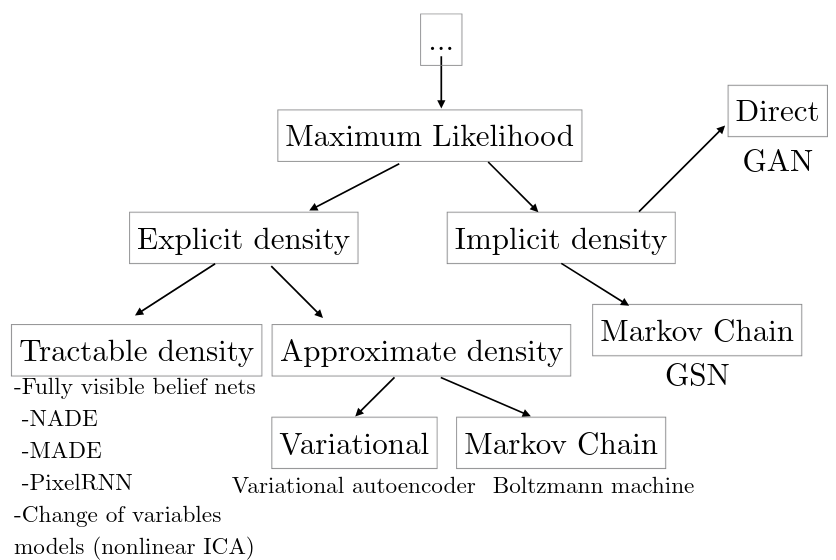
\includegraphics[width=0.8\textwidth]{images/taxonomy.png}}

\end{frame}

\begin{frame}{Applications: Image Recovery}
\protect\hypertarget{applications-image-recovery}{}

\begin{itemize}
\tightlist
\item
  We can upscale images, denoise them, fill/recover missing parts
  (inpainting)
\item
  In this case, we model \(p(x|\tilde{x})\) where \(\tilde{x}\) is \(x\)
  with some information destroyed ,e.g.~by blurring or noise
  introduction, and we would like to recover that information
\item
  Examples: TecoGAN (Chu et al. 2020), DeblurGAN (Kupyn et al. 2018),
  Palette (Saharia et al. 2021)
\end{itemize}

\center{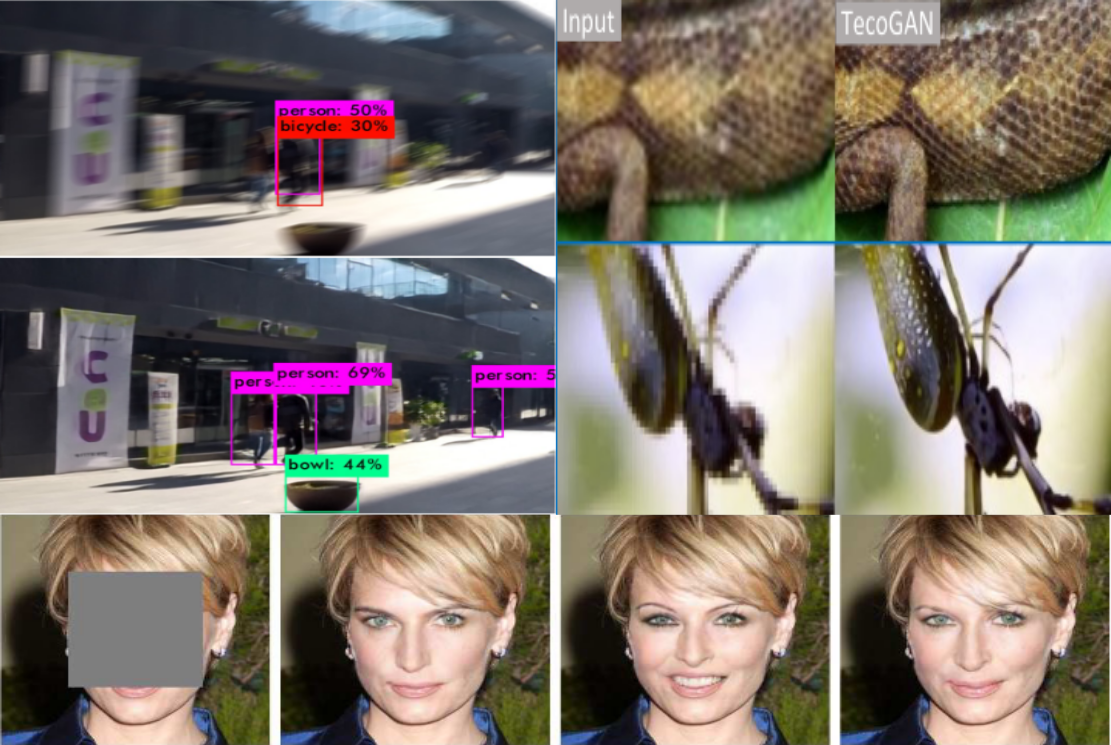
\includegraphics[width=0.35\textwidth]{images/image_recovery.png}}

\end{frame}

\begin{frame}{Applications: Conditional Image Generation}
\protect\hypertarget{applications-conditional-image-generation}{}

\begin{itemize}
\tightlist
\item
  We can generate images based on labels, or feature vectors, or natural
  language
\item
  In this case, we model \(p(x|y)\), where \(x\) is the image and \(y\)
  is the label, represented as a feature vector, a category, or a
  sequence of tokens (\(y=y_1,...,y_m\), where \(m\) is the number of
  tokens)
\end{itemize}

\center{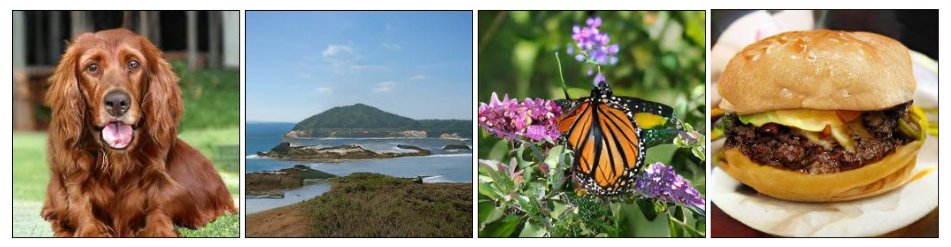
\includegraphics[width=0.8\textwidth]{images/biggan.png}}

(Brock, Donahue, and Simonyan 2019)

\end{frame}

\begin{frame}{Applications: Conditional Image Generation}
\protect\hypertarget{applications-conditional-image-generation-1}{}

\begin{itemize}
\tightlist
\item
  What would a ``penguin made of apples'' look like?
\end{itemize}

\center{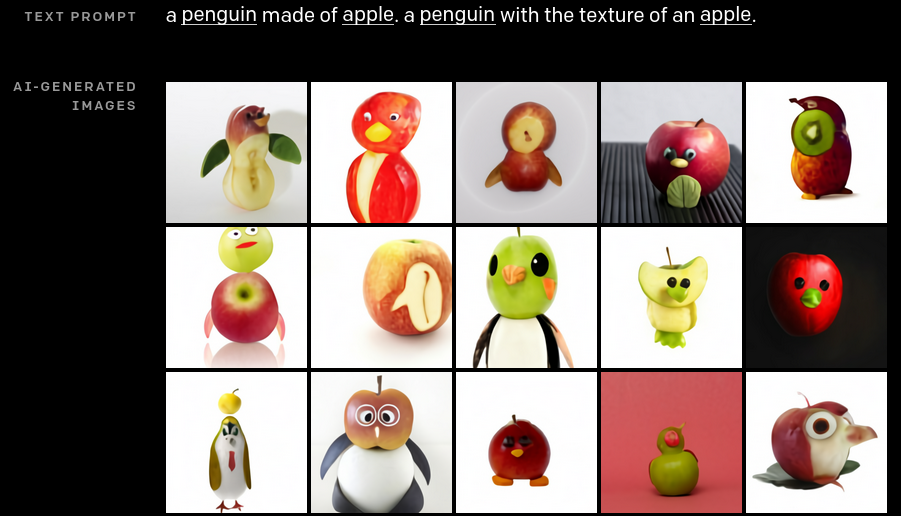
\includegraphics[width=0.7\textwidth]{images/DALL_e.png}}

OpenAI's DALL-E \url{https://openai.com/blog/dall-e/}, also see GLIDE
(Nichol et al. 2021)

\end{frame}

\begin{frame}{Applications: Image-to-Image Models}
\protect\hypertarget{applications-image-to-image-models}{}

\begin{itemize}
\tightlist
\item
  We can learn a mapping from images to images or from videos to videos,
  either with paired samples or unpaired ones. Examples: Pix2Pix (Isola
  et al. 2018), CycleGAN (Zhu et al. 2020), Pix2PixHD (Wang et al.
  2018), SPADE (Park et al. 2019), StarGANv2 (Choi et al. 2020), Palette
  (Saharia et al. 2021)
\end{itemize}

\center{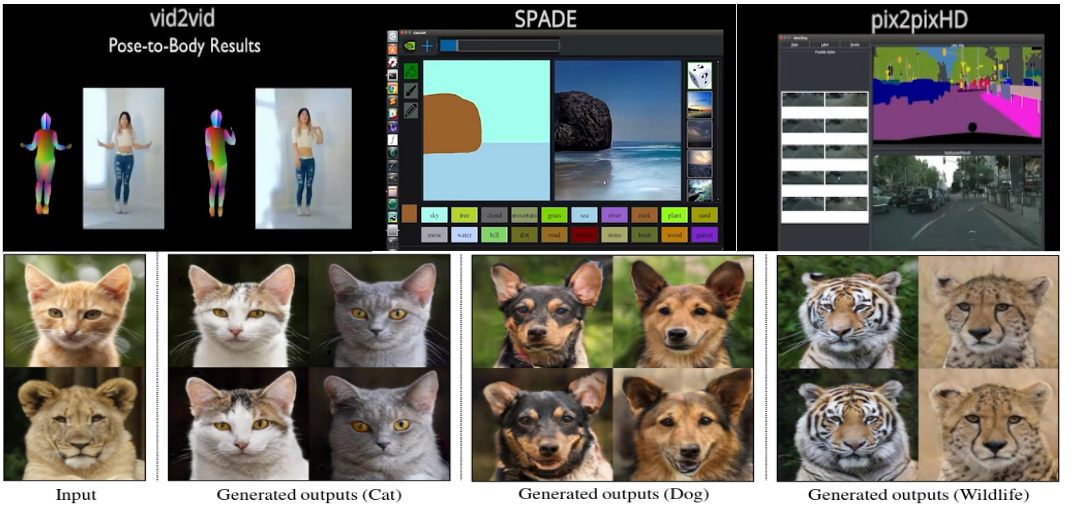
\includegraphics[width=0.7\textwidth]{images/image_to_image.png}}

\end{frame}

\begin{frame}{Applications: Speech Synthesis}
\protect\hypertarget{applications-speech-synthesis}{}

\begin{itemize}
\tightlist
\item
  WaveNet
\end{itemize}

\center{
\includegraphics[width=0.8\textwidth]{images/speech.png}}

(Oord et al. 2016)

\begin{itemize}
\tightlist
\item
  Tacotron2
\end{itemize}

\center{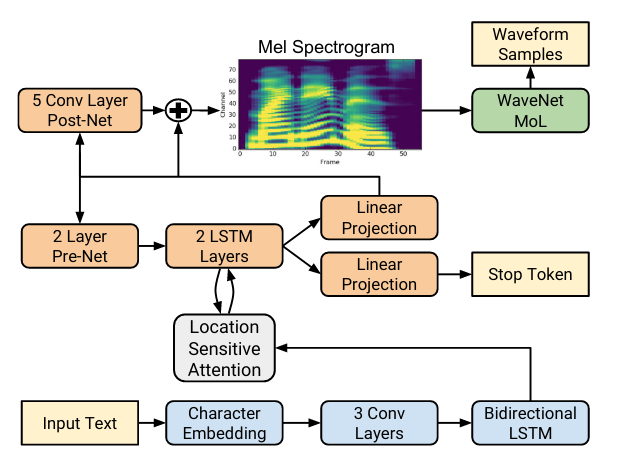
\includegraphics[width=0.3\textwidth]{images/tacotron2.png}}

(Shen et al. 2018)

\end{frame}

\begin{frame}{Applications: Music generation}
\protect\hypertarget{applications-music-generation}{}

\begin{itemize}
\tightlist
\item
  Jukebox (\url{https://openai.com/blog/jukebox/})
\end{itemize}

\center{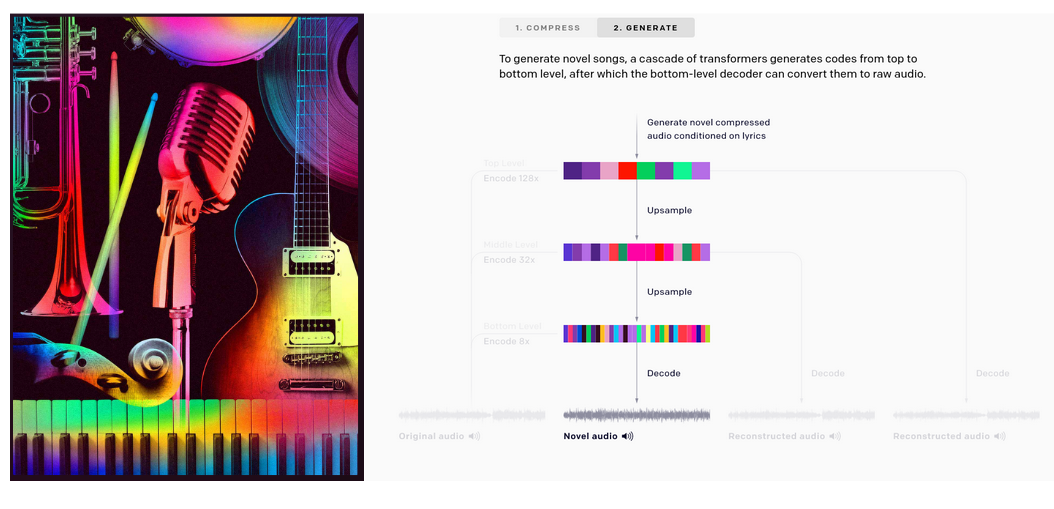
\includegraphics[width=0.9\textwidth]{images/jukebox.png}}

(Dhariwal et al. 2020)

\end{frame}

\begin{frame}{Applications: Text generation}
\protect\hypertarget{applications-text-generation}{}

\begin{itemize}
\tightlist
\item
  GPT-3 (Brown et al. 2020)
\end{itemize}

\center{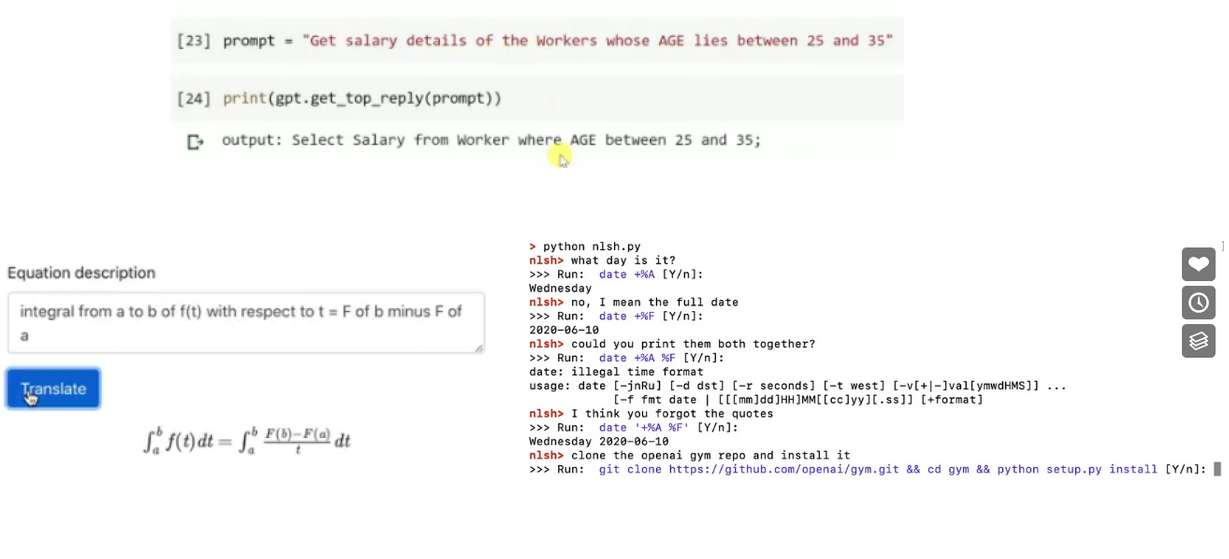
\includegraphics[width=0.9\textwidth]{images/gpt3_examples.png}}

Source: \url{https://bit.ly/3tqM8Sr}, \url{https://bit.ly/39KHNSe},
\url{https://bit.ly/3tvipHR}

\end{frame}

\begin{frame}{Applications: Reinforcement Learning}
\protect\hypertarget{applications-reinforcement-learning}{}

\begin{itemize}
\tightlist
\item
  We can simulate possible futures given the past. Application for
  reinforcement learning: learning world models and planning
\end{itemize}

\center{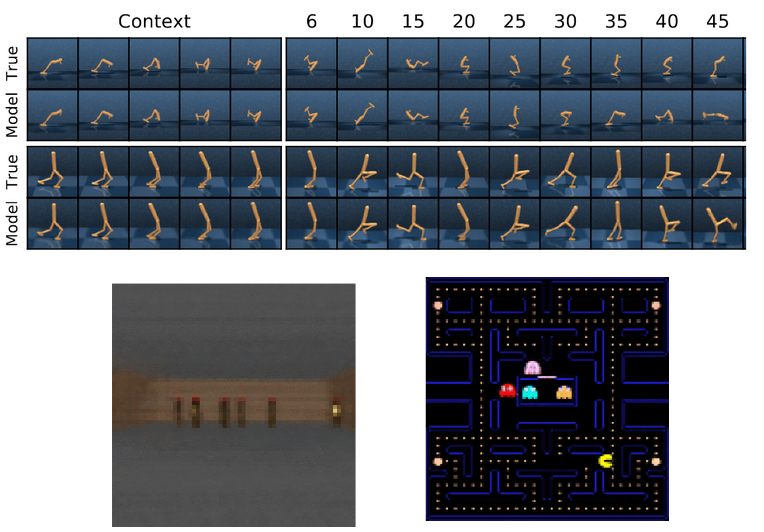
\includegraphics[height=6cm]{images/reinforcement_learning.png}}

(Hafner et al. 2020), (Kim et al. 2020)

\end{frame}

\begin{frame}{Generative Adversarial Networks}
\protect\hypertarget{generative-adversarial-networks}{}

\begin{itemize}
\tightlist
\item
  We have samples from a probability distribution \(p\), and we would
  like to learn a generator model that generates samples from
  \(x \sim p(x)\)
\item
  Discriminator is trained to distinguish between real and generated
  samples
\item
  Generator is trained to fool the discriminator 
\end{itemize}

\center{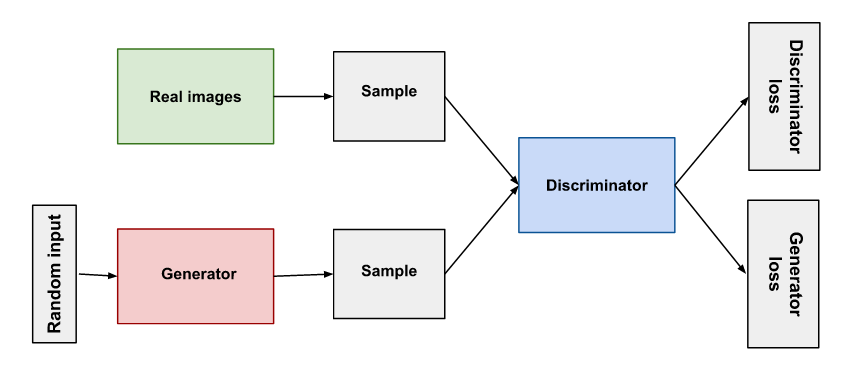
\includegraphics[width=0.7\textwidth]{images/gan.png}}

\end{frame}

\begin{frame}{Generative Adversarial Networks -- Formulation}
\protect\hypertarget{generative-adversarial-networks-formulation}{}

\[ \min _{G} \max _{D} \left[\mathbb{E}_{\boldsymbol{x} \sim p_{\text {data}}(\boldsymbol{x})}[\log D(\boldsymbol{x})]+\mathbb{E}_{\boldsymbol{z} \sim p_{\boldsymbol{z}}(\boldsymbol{z})}[\log (1-D(G(\boldsymbol{z})))]\right] \]

\begin{itemize}
\tightlist
\item
  \(D(x)\): probability that an image is real
\item
  \(D(G(z))\): probabilty that a generated image is real, where
  \(z \sim \mathbb{N}(0, 1)\)
\item
  \(\mathbb{E}_{\boldsymbol{x} \sim p_{\text {data}}(\boldsymbol{x})}[\log D(\boldsymbol{x})]\):
  discriminator on real data
\item
  \(\mathbb{E}_{\boldsymbol{z} \sim p_{\boldsymbol{z}}(\boldsymbol{z})}[\log (1-D(G(\boldsymbol{z})))]\):
  discriminator on generated data
\end{itemize}

\end{frame}

\begin{frame}{Generative Adversarial Networks -- Ideal Case}
\protect\hypertarget{generative-adversarial-networks-ideal-case}{}

\begin{itemize}
\tightlist
\item
  Generative Adversarial Networks (Goodfellow et al. 2014) shows that
  for a fixed generator \(G\), the optimal discriminator is:
  \(D^{*}_{G}(x) = \frac{p_{\text{data}}(x)}{p_{\text{data}} + p_{g}(x)}\)
\item
  They also show that the global optimal solution of the problem
  minimizes:
  \(-\log 4 + 2 \cdot \text{JSD}(p_{\text{data}} \parallel p_g )\),
  where the \(\text{JSD}\) is a measure between probability
  distributions
\item
  Since the \(\text{JSD}\) is non-negative, the globally optimal
  solution for the generator is the data distribution
  \(p_g = p_{\text{data}}\)
\end{itemize}

\end{frame}

\begin{frame}{Generative Adversarial Networks -- Training}
\protect\hypertarget{generative-adversarial-networks-training}{}

\begin{itemize}
\tightlist
\item
  In practice, we alternate between updating the generator and updating
  the discriminator
\end{itemize}

\center{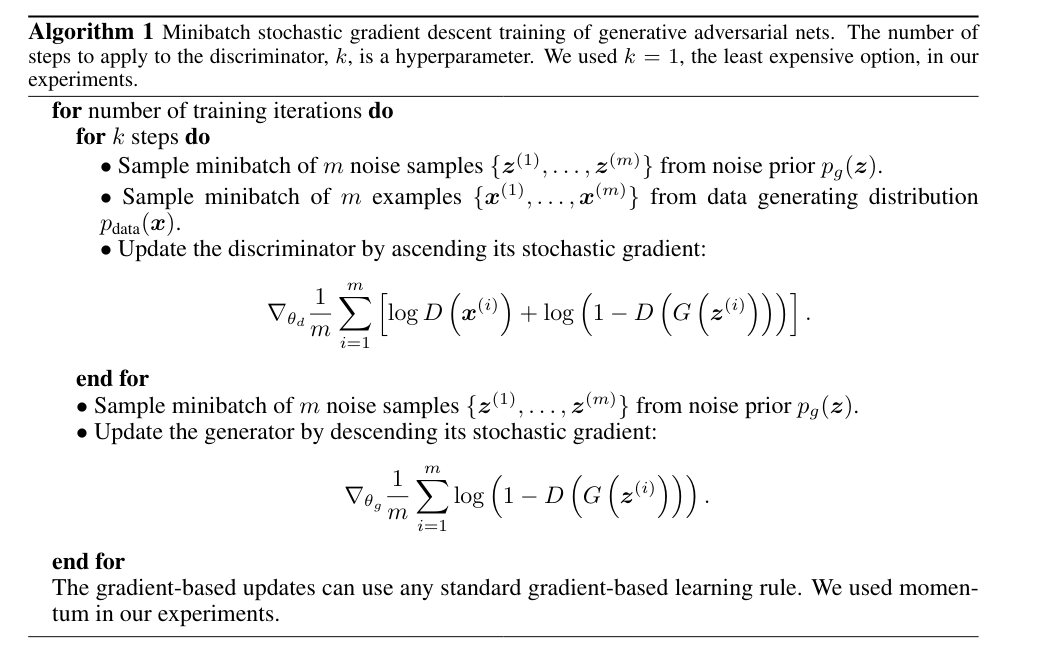
\includegraphics[height=5cm]{images/gan_training.png}}

\begin{itemize}
\tightlist
\item
  Note that in practice, for the generator they maximize
  \(\log (D(G(\boldsymbol{z})))\) instead of minimizing
  \(\log (1-D(G(\boldsymbol{z})))\), because it provides better
  gradients
\end{itemize}

\end{frame}

\begin{frame}{Generative Adversarial Networks -- Issues}
\protect\hypertarget{generative-adversarial-networks-issues}{}

\begin{itemize}
\tightlist
\item
  Non-convergence
\item
  Mode collapse
\item
  Vanishing gradient
\end{itemize}

\center{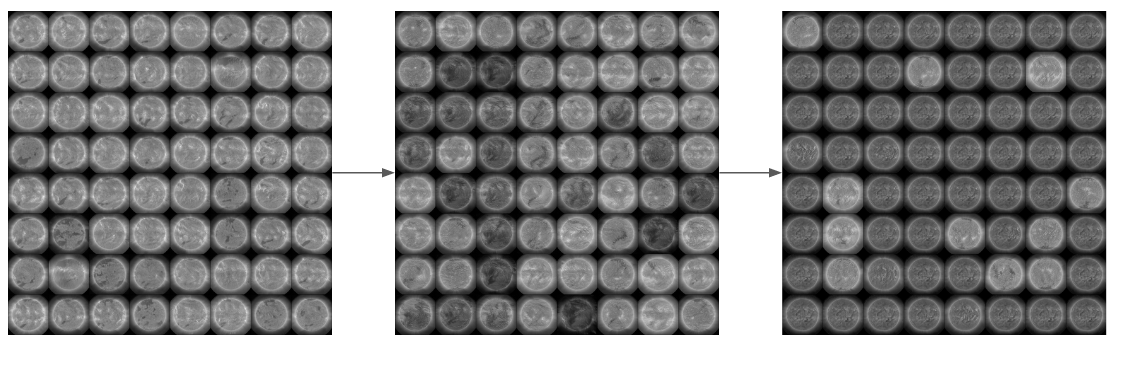
\includegraphics[width=0.9\textwidth]{images/collapse.png}}

(Illustration of mode collapse)

\end{frame}

\begin{frame}{The DCGAN Architecture}
\protect\hypertarget{the-dcgan-architecture}{}

\begin{itemize}
\tightlist
\item
  Removed fully connected layers: fully convolutional architecture for
  generator and discriminator
\item
  Uses batch normalization to stabilize training
\item
  One of the first architectures that worked well in practice on several
  datasets
  \center{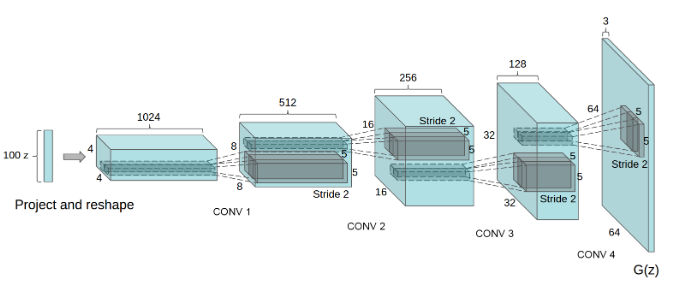
\includegraphics[width=0.9\textwidth]{images/dcgan.png}}
\end{itemize}

\end{frame}

\begin{frame}{The DCGAN Architecture -- Vector Arithmetics}
\protect\hypertarget{the-dcgan-architecture-vector-arithmetics}{}

\begin{itemize}
\tightlist
\item
  Interpretable directions in the latent space
\end{itemize}

\center{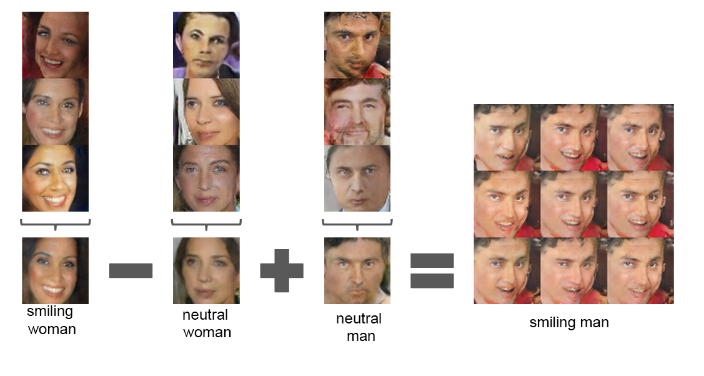
\includegraphics[width=0.9\textwidth]{images/dcgan_vector_arithmetics.png}}

\end{frame}

\begin{frame}{The DCGAN Architecture -- Interpolation in Latent Space}
\protect\hypertarget{the-dcgan-architecture-interpolation-in-latent-space}{}

\begin{itemize}
\tightlist
\item
  Smooth interpolation between generated images using the latent space
\end{itemize}

\center{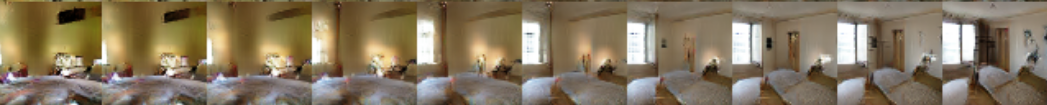
\includegraphics[width=0.9\textwidth]{images/dcgan_interp1.png}}

\center{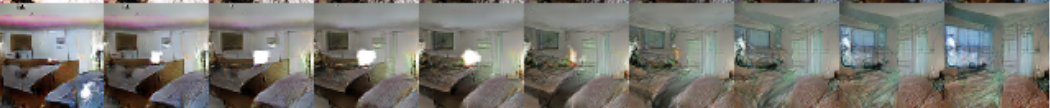
\includegraphics[width=0.9\textwidth]{images/dcgan_interp2.png}}

\end{frame}

\begin{frame}{Evaluation Metrics}
\protect\hypertarget{evaluation-metrics}{}

\begin{itemize}
\tightlist
\item
  In general, it's still an open question how to evaluate a generative
  model; in a lot of cases human visualization is still needed
\item
  In the ideal case, metrics should be task-specific (Theis, Oord, and
  Bethge 2016) and evaluate your generative model depending on how you
  will use it
\item
  Most common metrics used: Fréchet Inception Distance (FID) (Heusel et
  al. 2018), Inception Score (Salimans et al. 2016), precision and
  recall (Kynkäänniemi et al. 2019)
\end{itemize}

\end{frame}

\begin{frame}{Summary}
\protect\hypertarget{summary}{}

\begin{itemize}
\tightlist
\item
  Impressive progress during last years
\item
  Model sizes and data are getting bigger
\item
  Lot of different applications: image generation, text generation,
  speech synthesis, and more
\end{itemize}

\end{frame}

\begin{frame}[allowframebreaks]{References}
\protect\hypertarget{references}{}

\hypertarget{refs}{}
\leavevmode\hypertarget{ref-brock2019large}{}%
Brock, Andrew, Jeff Donahue, and Karen Simonyan. 2019. ``Large Scale Gan
Training for High Fidelity Natural Image Synthesis.''
\url{http://arxiv.org/abs/1809.11096}.

\leavevmode\hypertarget{ref-brown2020language}{}%
Brown, Tom B., Benjamin Mann, Nick Ryder, Melanie Subbiah, Jared Kaplan,
Prafulla Dhariwal, Arvind Neelakantan, et al. 2020. ``Language Models
Are Few-Shot Learners.'' \url{http://arxiv.org/abs/2005.14165}.

\leavevmode\hypertarget{ref-choi2020stargan}{}%
Choi, Yunjey, Youngjung Uh, Jaejun Yoo, and Jung-Woo Ha. 2020. ``StarGAN
V2: Diverse Image Synthesis for Multiple Domains.''
\url{http://arxiv.org/abs/1912.01865}.

\leavevmode\hypertarget{ref-Chu_2020}{}%
Chu, Mengyu, You Xie, Jonas Mayer, Laura Leal-Taixé, and Nils Thuerey.
2020. ``Learning Temporal Coherence via Self-Supervision for Gan-Based
Video Generation.'' \emph{ACM Transactions on Graphics} 39 (4).
\url{https://doi.org/10.1145/3386569.3392457}.

\leavevmode\hypertarget{ref-dhariwal2020jukebox}{}%
Dhariwal, Prafulla, Heewoo Jun, Christine Payne, Jong Wook Kim, Alec
Radford, and Ilya Sutskever. 2020. ``Jukebox: A Generative Model for
Music.'' \url{http://arxiv.org/abs/2005.00341}.

\leavevmode\hypertarget{ref-goodfellow2014generative}{}%
Goodfellow, Ian J., Jean Pouget-Abadie, Mehdi Mirza, Bing Xu, David
Warde-Farley, Sherjil Ozair, Aaron Courville, and Yoshua Bengio. 2014.
``Generative Adversarial Networks.''
\url{http://arxiv.org/abs/1406.2661}.

\leavevmode\hypertarget{ref-hafner2020dream}{}%
Hafner, Danijar, Timothy Lillicrap, Jimmy Ba, and Mohammad Norouzi.
2020. ``Dream to Control: Learning Behaviors by Latent Imagination.''
\url{http://arxiv.org/abs/1912.01603}.

\leavevmode\hypertarget{ref-heusel2018gans}{}%
Heusel, Martin, Hubert Ramsauer, Thomas Unterthiner, Bernhard Nessler,
and Sepp Hochreiter. 2018. ``GANs Trained by a Two Time-Scale Update
Rule Converge to a Local Nash Equilibrium.''
\url{http://arxiv.org/abs/1706.08500}.

\leavevmode\hypertarget{ref-isola2018imagetoimage}{}%
Isola, Phillip, Jun-Yan Zhu, Tinghui Zhou, and Alexei A. Efros. 2018.
``Image-to-Image Translation with Conditional Adversarial Networks.''
\url{http://arxiv.org/abs/1611.07004}.

\leavevmode\hypertarget{ref-karras2020training}{}%
Karras, Tero, Miika Aittala, Janne Hellsten, Samuli Laine, Jaakko
Lehtinen, and Timo Aila. 2020. ``Training Generative Adversarial
Networks with Limited Data.'' \url{http://arxiv.org/abs/2006.06676}.

\leavevmode\hypertarget{ref-kim2020learning}{}%
Kim, Seung Wook, Yuhao Zhou, Jonah Philion, Antonio Torralba, and Sanja
Fidler. 2020. ``Learning to Simulate Dynamic Environments with
Gamegan.'' \url{http://arxiv.org/abs/2005.12126}.

\leavevmode\hypertarget{ref-kupyn2018deblurgan}{}%
Kupyn, Orest, Volodymyr Budzan, Mykola Mykhailych, Dmytro Mishkin, and
Jiri Matas. 2018. ``DeblurGAN: Blind Motion Deblurring Using Conditional
Adversarial Networks.'' \url{http://arxiv.org/abs/1711.07064}.

\leavevmode\hypertarget{ref-kynkuxe4uxe4nniemi2019improved}{}%
Kynkäänniemi, Tuomas, Tero Karras, Samuli Laine, Jaakko Lehtinen, and
Timo Aila. 2019. ``Improved Precision and Recall Metric for Assessing
Generative Models.'' \url{http://arxiv.org/abs/1904.06991}.

\leavevmode\hypertarget{ref-nichol2021glide}{}%
Nichol, Alex, Prafulla Dhariwal, Aditya Ramesh, Pranav Shyam, Pamela
Mishkin, Bob McGrew, Ilya Sutskever, and Mark Chen. 2021. ``Glide:
Towards Photorealistic Image Generation and Editing with Text-Guided
Diffusion Models.'' \emph{arXiv Preprint arXiv:2112.10741}.

\leavevmode\hypertarget{ref-oord2016wavenet}{}%
Oord, Aaron van den, Sander Dieleman, Heiga Zen, Karen Simonyan, Oriol
Vinyals, Alex Graves, Nal Kalchbrenner, Andrew Senior, and Koray
Kavukcuoglu. 2016. ``WaveNet: A Generative Model for Raw Audio.''
\url{http://arxiv.org/abs/1609.03499}.

\leavevmode\hypertarget{ref-park2019semantic}{}%
Park, Taesung, Ming-Yu Liu, Ting-Chun Wang, and Jun-Yan Zhu. 2019.
``Semantic Image Synthesis with Spatially-Adaptive Normalization.''
\url{http://arxiv.org/abs/1903.07291}.

\leavevmode\hypertarget{ref-saharia2021palette}{}%
Saharia, Chitwan, William Chan, Huiwen Chang, Chris A Lee, Jonathan Ho,
Tim Salimans, David J Fleet, and Mohammad Norouzi. 2021. ``Palette:
Image-to-Image Diffusion Models.'' \emph{arXiv Preprint
arXiv:2111.05826}.

\leavevmode\hypertarget{ref-salimans2016improved}{}%
Salimans, Tim, Ian Goodfellow, Wojciech Zaremba, Vicki Cheung, Alec
Radford, and Xi Chen. 2016. ``Improved Techniques for Training Gans.''
\url{http://arxiv.org/abs/1606.03498}.

\leavevmode\hypertarget{ref-shen2018natural}{}%
Shen, Jonathan, Ruoming Pang, Ron J. Weiss, Mike Schuster, Navdeep
Jaitly, Zongheng Yang, Zhifeng Chen, et al. 2018. ``Natural Tts
Synthesis by Conditioning Wavenet on Mel Spectrogram Predictions.''
\url{http://arxiv.org/abs/1712.05884}.

\leavevmode\hypertarget{ref-theis2016note}{}%
Theis, Lucas, Aäron van den Oord, and Matthias Bethge. 2016. ``A Note on
the Evaluation of Generative Models.''
\url{http://arxiv.org/abs/1511.01844}.

\leavevmode\hypertarget{ref-wang2018highresolution}{}%
Wang, Ting-Chun, Ming-Yu Liu, Jun-Yan Zhu, Andrew Tao, Jan Kautz, and
Bryan Catanzaro. 2018. ``High-Resolution Image Synthesis and Semantic
Manipulation with Conditional Gans.''
\url{http://arxiv.org/abs/1711.11585}.

\leavevmode\hypertarget{ref-zhu2020unpaired}{}%
Zhu, Jun-Yan, Taesung Park, Phillip Isola, and Alexei A. Efros. 2020.
``Unpaired Image-to-Image Translation Using Cycle-Consistent Adversarial
Networks.'' \url{http://arxiv.org/abs/1703.10593}.

\end{frame}


\end{document}
